\documentclass[a4paper,14pt]{extreport}
\usepackage[left=1.5cm,right=1.5cm,
    top=1.5cm,bottom=2cm,bindingoffset=0cm]{geometry}
\usepackage{scrextend}
\usepackage[T1,T2A]{fontenc}
\usepackage[utf8]{inputenc}
\usepackage[english,russian,ukrainian]{babel}
\usepackage{tabularx}
\usepackage{amssymb}
\usepackage{color}
\usepackage{amsmath}
\usepackage{mathrsfs}
\usepackage{listings}
\usepackage{graphicx}
\graphicspath{ {./images/} }
\usepackage{lipsum}
\usepackage{xcolor}
\usepackage{hyperref}
\usepackage{tcolorbox}
\usepackage{tikz}
\usepackage[framemethod=TikZ]{mdframed}
\usepackage{wrapfig,boxedminipage,lipsum}
\mdfdefinestyle{MyFrame}{%
linecolor=blue,outerlinewidth=2pt,roundcorner=20pt,innertopmargin=\baselineskip,innerbottommargin=\baselineskip,innerrightmargin=20pt,innerleftmargin=20pt,backgroundcolor=gray!50!white}
 \usepackage{csvsimple}
 \usepackage{supertabular}
\usepackage{pdflscape}
\usepackage{fancyvrb}
%\usepackage{comment}
\usepackage{array,tabularx}
\usepackage{colortbl}

\usepackage{varwidth}
\tcbuselibrary{skins}
\usepackage{fancybox}


\usepackage{tikz}
\usepackage[framemethod=TikZ]{mdframed}
\usepackage{xcolor}
\usetikzlibrary{calc}
\makeatletter
\newlength{\mylength}
\xdef\CircleFactor{1.1}
\setlength\mylength{\dimexpr\f@size pt}
\newsavebox{\mybox}
\newcommand*\circled[2][draw=blue]{\savebox\mybox{\vbox{\vphantom{WL1/}#1}}\setlength\mylength{\dimexpr\CircleFactor\dimexpr\ht\mybox+\dp\mybox\relax\relax}\tikzset{mystyle/.style={circle,#1,minimum height={\mylength}}}
\tikz[baseline=(char.base)]
\node[mystyle] (char) {#2};}
\makeatother

\definecolor{ggreen}{rgb}{0.4,1,0}
\definecolor{rred}{rgb}{1,0.1,0.1}
\definecolor{amber}{rgb}{1.0, 0.75, 0.0}
\definecolor{babyblue}{rgb}{0.54, 0.81, 0.94}
\definecolor{asparagus}{rgb}{0.53, 0.66, 0.42}
\definecolor{chartreuse}{rgb}{0.5, 1.0, 0.0}
\definecolor{darkorchid}{rgb}{0.6, 0.2, 0.8}

\usepackage{float}
\usepackage{wrapfig}
\usepackage{framed}
%for nice Code{
\lstdefinestyle{customc}{
  belowcaptionskip=1\baselineskip,
  breaklines=true,
  frame=L,
  xleftmargin=\parindent,
  language=C,
  showstringspaces=false,
  basicstyle=\small\ttfamily,
  keywordstyle=\bfseries\color{green!40!black},
  commentstyle=\itshape\color{purple!40!black},
  identifierstyle=\color{blue},
  stringstyle=\color{orange},
}
\lstset{escapechar=@,style=customc}
%}


\begin{document}
\pagecolor{white}

%----------------------------------------1
\newtcbox{\xmybox}[1][red]{on line, arc=7pt,colback=#1!10!white,colframe=#1!50!black, before upper={\rule[3pt] {0pt}{10pt}},boxrule=1pt,boxsep=0pt,left=6pt,right=6pt,top=2pt,bottom=2pt}

\begin{center}\xmybox[green]{Mnatsakanov Anton} \xmybox[amber]{DP-82} \xmybox[blue]{Variant №5}
\vspace{1cm}

\end{center}


\begin{center}Як математично і графічно описуються діелектричні втрати від релаксаційної поляризації?\end{center}

Dielectric losses caused by thermal polarization. Thermal polarization is essentially reduced to electrodiffusion, in which charges (or dipoles)
are asymmetrically $ \quad $ accumulated reoriented). The thermal motion causes the polarization to be established relatively slowly (see Section Three). The relaxation time of thermal polarization depends on temperature and under normal conditions (at $ 300 \mathrm {~ K}) $ is usually $ 10^{- 3} -10^{- 9} $ s. It is this range of frequencies that coincides with the
range of use of dielectrics in electrical and electronic engineering (50 Hz ... 100 GHz)

Therefore, thermal polarization is precisely what leads to undesirable dielectric losses in most technical uses of dielectrics. Elastic (deformation) polarization is too
 fast a process to affect losses in the 50 Hz ... 100 GHz. It should be noted that migratory (volume charge) polarization is a
  slower mechanism that leads to instabilities $ \varepsilon (\omega, T) $ and dielectric losses at infralow frequencies $ (10^{- 3} \ldots 10^{2}  $ Hz $) $
The dielectric contribution of both relaxation and migration polarization depends on frequency and is described by Debye's equation:
$$
\varepsilon^{*}(\omega) \varepsilon^{\prime} -i \varepsilon^{\prime \prime} = \varepsilon(\infty) + \frac{\varepsilon (0) - \varepsilon (\infty)} {1 + i \omega \tau}
$$

where $ \varepsilon (0) $ and $ \varepsilon (\infty) $ are the values of dielectric permittivity at low and high frequencies respectively compared to the dispersion frequency $ \omega = \omega {\text {rel}} = 1 / \tau $, where $ \tau $ relaxation time. The main parameters characterizing the relaxation losses are shown in Fig. \ref{ris1}. From them it is possible to analyze the frequency dependence


of the parameters $ \varepsilon ^ {\prime} \varepsilon ^ {\prime \prime} $ i $  tg \delta. $ In low frequency case $ (\omega \rightarrow 0) $ dielectric permittivity
$ \varepsilon ^ {\prime} = \varepsilon (0), $ and at high frequency $ (\omega \rightarrow \infty) \varepsilon ^ {\prime} = \varepsilon (\infty). $ If the frequency $ \omega = 1 / \tau $
the dielectric contribution $ \varepsilon (0) - \varepsilon (\infty) $ is exactly halved (Fig. \ref{ris1},  a). 3
The absence of conductivity $ \varepsilon ^ {\prime \prime} = 0 $ both at low frequencies (when $ \omega \rightarrow 0 $) and at
high (when $ \omega \rightarrow \infty$). It is easy to show that $ \varepsilon ^ {\prime \prime} (\omega) $ has a maximum at the frequency of  $\omega $ =
$ 1 / \tau, $ that is, at a frequency where the contribution of $ \varepsilon_{\text {rel}} $ is halved (Fig. \ref{ris1},  б).
The frequency dependence of tg $ \delta $ is also characterized by a maximum:
$$
tg \delta_{\mathrm {max}} = \frac{\varepsilon (0) - \varepsilon (\infty)} {2 \sqrt {\varepsilon (0) \varepsilon (\infty)}}; \omega_{\mathrm {tg} \delta_{\mathrm {max}}} = \frac {1} {\tau} \sqrt {\frac {\varepsilon (0)} {\varepsilon (\infty)}}
$$
This maximum is observed at a slightly higher frequency than the maximum $ \varepsilon ^ {\prime} $
$ ($ Fig. \ref{ris1},  г $) $

From the formula for the specific power of dielectric losses $ p $ for the relaxation polarization, it follows that in the case of low frequencies, when the relaxation polarization
has time to settle in time, dielectric losses are almost undetectable. If the dispersion frequency is $ \omega = 1 / \tau, $ then $ p = 0.5 g E^{2}, $ where the parameter $ g = \ alpha_{\mathrm {I}} \tau \varepsilon_ {0} is $
reactive conductivity. At high frequencies, when $ \omega \tau> 1, $ losses reach a maximum value equal to $ g E ^ {2}, $ and further do not depend on frequency increase (Fig. 5.5,6). So, although the relaxation polarization is delayed and no longer makes a dielectric contribution, the specific loss power from the relaxation processes remains maximum. Therefore, for example, to develop
high-frequency and low-frequency dielectrics of impurity and defect
structures that cause low-frequency relaxation are extremely undesirable,
because they do not noticeably affect the value of $ \varepsilon, $ significantly increase
losses.



The temperature dependences $ \varepsilon $ i tg $ \delta $ in the case of relaxation polarization are also characterized by maxima. According to the experimental data on the temperature dependences $tg \delta (T) $ i $\varepsilon (T) $ determine the height of the potential barrier U, which the particles (ions, dipoles or electrons) overcome during the relaxation process of edektrodiffusion. To calculate $ U $ it is sufficient to determine the temperatures $ T_ {1} $ and $ T_ {2} $ for the two frequencies $  (\omega_ {1}
$ i $\omega_ {2} ), $ which cause the maximum losses:
$$
U=\frac{k T_{1} T_{2}}{T_{2}-T_{1}} \ln \frac{\omega_{2}}{\omega_{1}}
$$





\begin{figure}[h]
\center{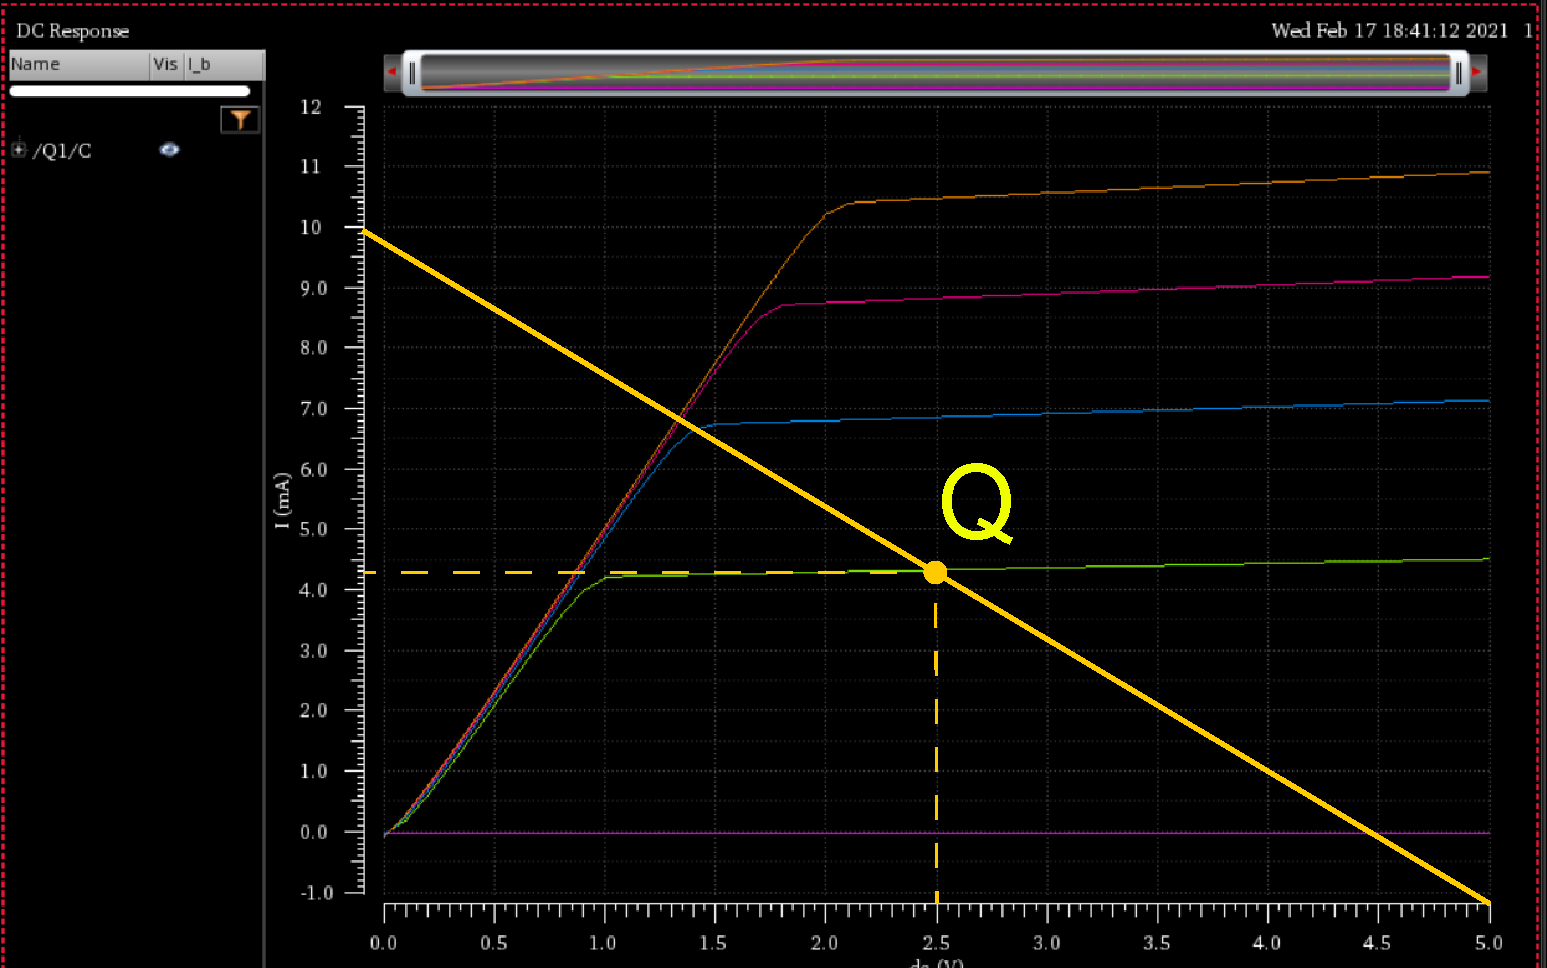
\includegraphics[width=0.9\linewidth]{1.png}}
\caption{Frequency dependences of dielectric constant (a), absorbed energy density (б), loss factor (в) and loss angle tangent (г) in dielectrics in which thermal polarization mechanisms predominate.}
\label{ris1}
\end{figure}
\end{document}
